%! TEX root = Programacion.tex

\documentclass{./Programacion.tex}

\begin{document}
\chapter{Python}
\section{Programación Orientada a Objetos (POO)}
Permite programar realizando abstracciones. Consiste en definir plantillas que desarrollan como cada \textbf{objeto} (instancias de las clases) definirá sus atributos y los diferentes métodos que estos tienen.
\begin{itemize}
	\item Clase:
		\begin{itemize}
			\item Atributos
			\item Métodos
		\end{itemize}
\end{itemize}
\subsection{Encapsulamiento}
Es el concepto de aislar el funcionamiento de los métodos y variables de una clase.
\section{Declaración de clases}
\begin{lstlisting}
	class Clase:
		pass

	objeto = Clase()
\end{lstlisting}
Cada clase tiene atributos predefinido, pero luego tenemos los atributos de \textbf{instancia}, que permite al usuario modificar los atributos en su creación:
\begin{lstlisting}[language=python]
	class Clase:
	def __init__(self, at1, at2):
		self.var1 = at1
		self.var2 = at2

	obj = Clase(1, 2)
	obj.var1 #1
	obj.var2 #2
\end{lstlisting}
Las diferencias entre ambos es que los atributos de clase se almacenan en los metadatos de la clase, mientras que los de instancia se guardan en los metadatos del objeto.
\subsection{Métodos}
Son funciones definidas dentro de una propia clase, y representan las acciones que cada instancia de dicha clase puede realizar. Estos métodos también pueden acceder a los atributos de una clase, por lo que es una forma de encapsular estos.
Existen dos tipos de métodos:
\begin{itemize}
	\item Métodos de instancia: relacionados con cada objeto.
	\item Métodos de clase: solo se pueden usar con la clase.
\end{itemize}
\section{Herencia y abstracción}
La herencia es un concepto fundamental de la OOP\@. Consiste en la creación de clases base, con una funcionalidad definida, y luego definir clases que \textbf{hereden} de esta, de forma que tengan toda la funcionalidad de la clase padre, además de nuevas funcionalidades que definamos en esta.
\begin{lstlisting}[language=python]
class Padre:
	def __init__(self):
		self.foo = bar

class Hija(Padre):
	def __init__(self):
		#Modificamos el valor de la clase padre
		self.bar = fizz

hija = Hija()
print(hija.foo) #bar
\end{lstlisting}
También podemos extender la funcionamiento de clases mediante \verb|super|:
\begin{lstlisting}[language=python]
def presentarse(self):
	super().presentarse() #Llamamos a la funcion de la clase padre
	# codigo
\end{lstlisting}
Además, también podemos ahorrarnos código para utilizar la función de definición de clases padre:
\begin{lstlisting}[language=python]
class Hija(Padre):
	def __init__(self, nombre, apellido, edad):
		super.__init__(nombre, apellido)
		self.edad = edad
\end{lstlisting}
También es posible hereder de múltiples clases:
\begin{lstlisting}[language=python]
class Clase_1:
	pass
class Clase_2:
	pass
class Clase_3(Clase_1, Clase_2):
	pass
\end{lstlisting}
\pagebreak
\section{Abstracción}
En la POO, una interfaz es una herramienta que define qué funcionalidades debe terne un cierto objeto. Una interfaz permite saber al desarrollador qué funcionalidad va a tener un objeto o clase, sin saber realmente cómo va a implementarla.\\
De esta misma forma, podemos utilizar las implementaciones que una interfaz nos garantiza que dicha herramienta va a tener.
\begin{figure}[ht]
	\centering

\tikzset{every picture/.style={line width=0.75pt}} %set default line width to 0.75pt

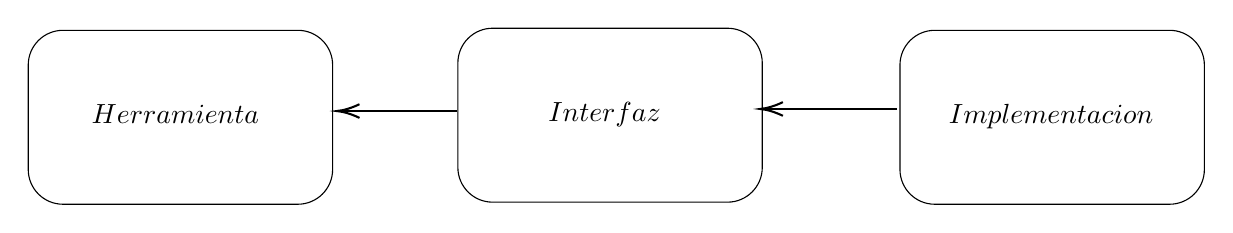
\begin{tikzpicture}[x=0.75pt,y=0.75pt,yscale=-1,xscale=1]
%uncomment if require: \path (0,300); %set diagram left start at 0, and has height of 300

%Rounded Rect [id:dp807997340687292]
\draw   (48.67,105.86) .. controls (48.67,96.6) and (56.17,89.1) .. (65.43,89.1) -- (178.57,89.1) .. controls (187.83,89.1) and (195.33,96.6) .. (195.33,105.86) -- (195.33,156.14) .. controls (195.33,165.4) and (187.83,172.9) .. (178.57,172.9) -- (65.43,172.9) .. controls (56.17,172.9) and (48.67,165.4) .. (48.67,156.14) -- cycle ;
%Rounded Rect [id:dp18101874602402723]
\draw   (255.67,104.86) .. controls (255.67,95.6) and (263.17,88.1) .. (272.43,88.1) -- (385.57,88.1) .. controls (394.83,88.1) and (402.33,95.6) .. (402.33,104.86) -- (402.33,155.14) .. controls (402.33,164.4) and (394.83,171.9) .. (385.57,171.9) -- (272.43,171.9) .. controls (263.17,171.9) and (255.67,164.4) .. (255.67,155.14) -- cycle ;
%Rounded Rect [id:dp419014409176622]
\draw   (468.67,105.86) .. controls (468.67,96.6) and (476.17,89.1) .. (485.43,89.1) -- (598.57,89.1) .. controls (607.83,89.1) and (615.33,96.6) .. (615.33,105.86) -- (615.33,156.14) .. controls (615.33,165.4) and (607.83,172.9) .. (598.57,172.9) -- (485.43,172.9) .. controls (476.17,172.9) and (468.67,165.4) .. (468.67,156.14) -- cycle ;
%Straight Lines [id:da8520844371735503]
\draw    (255.33,128) -- (199.33,128) ;
\draw [shift={(197.33,128)}, rotate = 360] [color={rgb, 255:red, 0; green, 0; blue, 0 }  ][line width=0.75]    (10.93,-3.29) .. controls (6.95,-1.4) and (3.31,-0.3) .. (0,0) .. controls (3.31,0.3) and (6.95,1.4) .. (10.93,3.29)   ;
%Straight Lines [id:da3598742136694002]
\draw    (467.33,127) -- (403.33,127) ;
\draw [shift={(401.33,127)}, rotate = 360] [color={rgb, 255:red, 0; green, 0; blue, 0 }  ][line width=0.75]    (10.93,-3.29) .. controls (6.95,-1.4) and (3.31,-0.3) .. (0,0) .. controls (3.31,0.3) and (6.95,1.4) .. (10.93,3.29)   ;

% Text Node
\draw (78,123.4) node [anchor=north west][inner sep=0.75pt]    {$Herramienta$};
% Text Node
\draw (298,122.4) node [anchor=north west][inner sep=0.75pt]    {$Interfaz$};
% Text Node
\draw (491,123.4) node [anchor=north west][inner sep=0.75pt]    {$Implementacion$};


\end{tikzpicture}
\caption{Interfaces}
\end{figure}
Sin embargo, las interfaces no existen en Python, por lo que las interfaces son equivalentes a clases padre con funciones vacía:
\begin{lstlisting}[language=python]
class Interfaz:
	def implementacion_1():
		pass
\end{lstlisting}
Esto es similar a las \textbf{clases abstractas}, que son clases que no se puende instanciar, sino que solo se puede derivar de ellas.\\
Para definir funciones abstractas en Python, utilizamos el decorador \verb|@abstractmethod|, y la clase debe empezar debe heredar de \verb|ABC|:
\begin{lstlisting}[language=python]
from abc import ABC, abstractmethod

class Abstract(ABC):
	@abstractmethod
	def funcionAbstracta(self):
		# codigo
\end{lstlisting}
\section{Archivos y operaciones}
\begin{itemize}
  \item CSV: permite hacer tablas, y es como una versión más ligera de Excel.
  \item JSON: JavaScript Object Notation
\end{itemize}
\section{Apertura de archivos}
Para llevar a cabo cualquier operación de archivos, utilizamos \verb|open|
\begin{lstlisting}[language=python]
open(file='ruta', mode= 'modo de apertura')
\end{lstlisting}
Los modos son:
\begin{itemize}
  \item \verb|w|: escritura
\item \verb|r|: lectura
\item \verb|a|: append, escritura y lectura.
\end{itemize}
Similarmente, para cerrar archivos, utilizamos \verb|archivo.close()|. Es necesario cerrar el archivo para que el sistema operativo recupere los recursos utilizados. En Python, existen los \verb|context managers|, que nos permiten agilizar este proceso:
\begin{lstlisting}[language=python]
with open("archivo.txt", "r") as archivo:
	#codigo
\end{lstlisting}
De esta forma, el archivo se cerrará automáticamente.
\section{Lectura y escritura}
Una vez abierto el archivo, podemos leerlo con:
\begin{itemize}
	\item \verb|file.read()|: lee todo el archivo.
	\item Podemos iterar por cada línea así:
		\begin{lstlisting}[language=python]
		for linea in file:
			print(linea.strip())
		\end{lstlisting}
\end{itemize}
Para escribir en el archivo:
\begin{lstlisting}[language=python]
texto = "Hola mundo"

with open("archivo.txt", "w") as file:
	file.write(texto)
\end{lstlisting}
\section{Archivos CSV}	
Para utilizarla, utilizarémos la librería \verb|csv|:
\begin{lstlisting}[language=python]
with open("archivo.csv", "r") as file:
	lectura = csv.reader(file)
	for linea in lectura:
		print(linea)
\end{lstlisting}
Para escribir en un archivo, utilizamos la clase \verb|writer|:
\begin{lstlisting}[language=python]
with open("archivo.csv", "w") as file:
	writer = csv.writer(file)
	for fila in datos:
		writer.writerow(fila)
\end{lstlisting}
\end{document}
